%%%%%%%%%%
% HEADER %
%%%%%%%%%%

\documentclass[
  10pt, 
  a4paper,
  oneside, 
  % twoside, 
  headinclude, 
  footinclude, 
  BCOR5mm, 
]{scrartcl}

% package
\usepackage[francais]{babel}
\usepackage{color}
\usepackage{enumitem}

\usepackage{minted}
\usemintedstyle{trac}
\definecolor{LightGray}{gray}{0.90}

\usepackage[pdftex]{graphicx}

\setlength{\parindent}{0cm}
\setlength{\parskip}{1ex plus 0.5ex minus 0.2ex}
\newcommand{\hsp}{\hspace{20pt}}
\newcommand{\HRule}{\rule{\linewidth}{0.5mm}}

\fvset{
  frame = lines,
  framesep = 2mm,
  baselinestretch = 1,
  rulecolor = \color{LightGray},
  fontsize = \normalsize,
  tabsize = 3,
}

%%%%%%%%%%%%%%%%%%%%%%%%%%%%%%%%%%%%%%%%%
% Arsclassica Article
% Structure Specification File
%
% This file has been downloaded from:
% http://www.LaTeXTemplates.com
%
% Original author:
% Lorenzo Pantieri (http://www.lorenzopantieri.net) with extensive modifications by:
% Vel (vel@latextemplates.com)
%
% License:
% CC BY-NC-SA 3.0 (http://creativecommons.org/licenses/by-nc-sa/3.0/)
%
%%%%%%%%%%%%%%%%%%%%%%%%%%%%%%%%%%%%%%%%%

%----------------------------------------------------------------------------------------
%	REQUIRED PACKAGES
%----------------------------------------------------------------------------------------

\usepackage[
nochapters, % Turn off chapters since this is an article        
beramono, % Use the Bera Mono font for monospaced text (\texttt)
eulermath,% Use the Euler font for mathematics
pdfspacing, % Makes use of pdftex’ letter spacing capabilities via the microtype package
dottedtoc % Dotted lines leading to the page numbers in the table of contents
]{classicthesis} % The layout is based on the Classic Thesis style

\usepackage{arsclassica} % Modifies the Classic Thesis package

\usepackage[T1]{fontenc} % Use 8-bit encoding that has 256 glyphs

\usepackage[utf8]{inputenc} % Required for including letters with accents

\usepackage{graphicx} % Required for including images
\graphicspath{{graphics/}} % Set the default folder for images

\usepackage{enumitem} % Required for manipulating the whitespace between and within lists

\usepackage{lipsum} % Used for inserting dummy 'Lorem ipsum' text into the template

\usepackage{subfig} % Required for creating figures with multiple parts (subfigures)

\usepackage{amsmath,amssymb,amsthm} % For including math equations, theorems, symbols, etc

\usepackage{varioref} % More descriptive referencing

%----------------------------------------------------------------------------------------
%	THEOREM STYLES
%---------------------------------------------------------------------------------------

\theoremstyle{definition} % Define theorem styles here based on the definition style (used for definitions and examples)
\newtheorem{definition}{Definition}

\theoremstyle{plain} % Define theorem styles here based on the plain style (used for theorems, lemmas, propositions)
\newtheorem{theorem}{Theorem}

\theoremstyle{remark} % Define theorem styles here based on the remark style (used for remarks and notes)

%----------------------------------------------------------------------------------------
%	HYPERLINKS
%---------------------------------------------------------------------------------------

\hypersetup{
%draft, % Uncomment to remove all links (useful for printing in black and white)
colorlinks=true, breaklinks=true, bookmarks=true,bookmarksnumbered,
urlcolor=webbrown, linkcolor=RoyalBlue, citecolor=webgreen, % Link colors
pdftitle={}, % PDF title
pdfauthor={\textcopyright}, % PDF Author
pdfsubject={}, % PDF Subject
pdfkeywords={}, % PDF Keywords
pdfcreator={pdfLaTeX}, % PDF Creator
pdfproducer={LaTeX with hyperref and ClassicThesis} % PDF producer
}

\hyphenation{Fortran hy-phen-ation}

\titleformat
  {\section}[block]
  {\sffamily\large\normalfont}
  {\thesection}
  {1em}
  {\Large\spacedlowsmallcaps}

\titleformat
  {\subsection}[block]
  {\sffamily\normalsize\normalfont}
  {\thesubsection}
  {1em}
  {}

% STYLE

\renewcommand{\sectionmark}[1]{\markright{\spacedlowsmallcaps{#1}}}
\lehead{\mbox{\llap{\small\thepage\kern1em\color{halfgray} \vline}\color{halfgray}\hspace{0.5em}\rightmark\hfil}}

\pagestyle{scrheadings}
\setcounter{tocdepth}{3}


% HEAD PAGE

\begin{document}

%\maketitle

\begin{titlepage}
  \begin{sffamily}
  \begin{center}
    \textsc{\LARGE Université de Fribourg} \\ [2cm]
    \textsc{\Large Very Deep Learning} \\ [2cm]

    % Title
    \HRule \\ [0.5cm]
    {\huge\spacedallcaps{Deepdraw} \\ [0.5cm]}
    \HRule \\ [2cm]
    
    \textsc{
    	\Large Ismaïl \spacedallcaps{Senhaji}, 
    	\Large Gil \spacedallcaps{Clavien} \\
    	\Large Noé \spacedallcaps{Zufferey}, 
    	\Large Michaël \spacedallcaps{Diatta} \\
    	\Large Igor \spacedallcaps{Dundic}} \\ [2cm]
    
    \textsc{\large \emph{Responsable} : Liwicky \spacedallcaps{Liwicky}} \\ [0.5cm]
    \textsc{\Large 20 décembre 2017} \\    

    \vfill

    % Bottom of the page
    Département d’Informatique — Departement für Informatik \\
    Université de Fribourg — Universität Freiburg \\
    Boulevard de Pérolles 90, 1700 Fribourg, Suisse
  \end{center}
  \end{sffamily}
\end{titlepage}

\newpage

% CONTENT

\section{Introduction}

For the very deep learning project, we decided to build, train and manage a neural network that can draw pictures of simple concept. We use the Quick Draw Dataset, a google's game, that provide a huge dataset of labelised simple drawing.

\section{About quickdraw-dataset}

The Quick Draw Dataset\footnote{\url{https://github.com/googlecreativelab/quickdraw-dataset}} is a collection of 50 million drawings across 345 categories, contributed by players of the game Quick, Draw!\footnote{\url{https://quickdraw.withgoogle.com/\#}}. The drawings were captured as timestamped vectors, tagged with metadata including what the player was asked to draw and in which country the player was located.

The Quick Draw game principle is to draw specific picture given by the computer. This one try to recognize, with machine learning, your drawing.

\begin{figure}[h]
	\center
	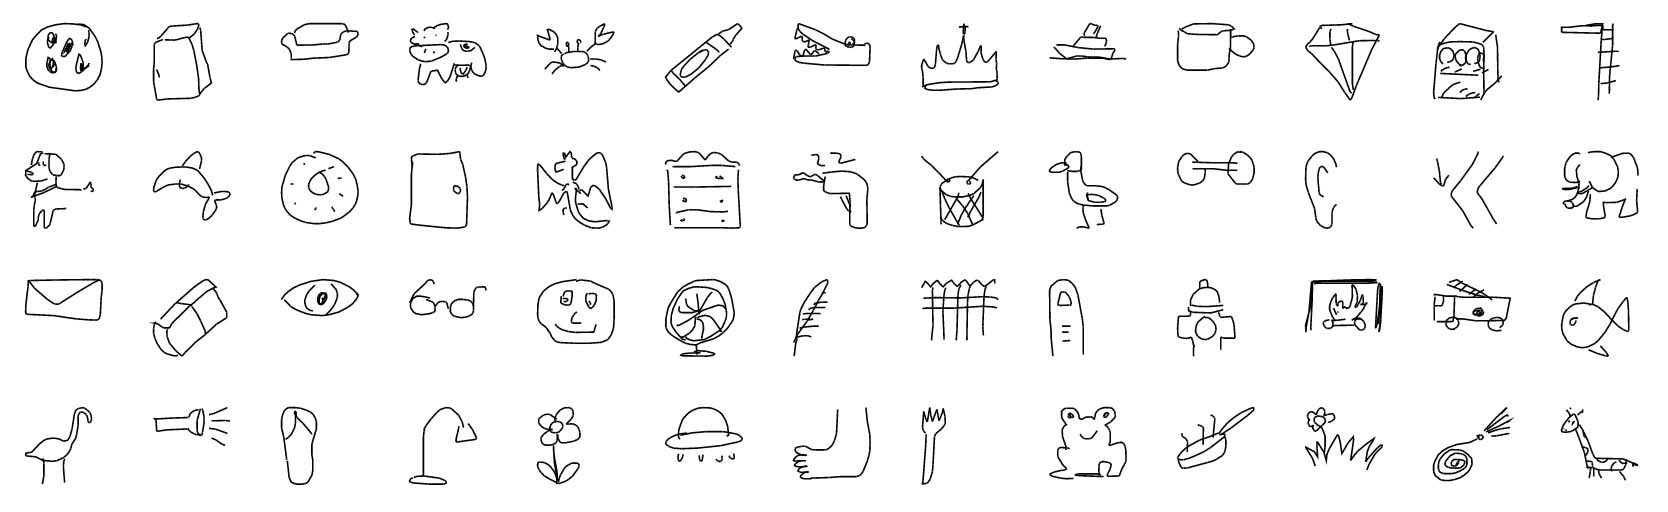
\includegraphics[width=\columnwidth]{qdd-example.jpg}
	\caption{Quick Draw example.}
	\label{promo-asylamba}
\end{figure}

The Quick Draw Dataset provides preprocessed dataset. We choose to use the \textbf{Simplified Drawing files} preprocessed dataset. They've simplified the vectors, removed the timing information, and positioned and scaled the data into a 256x256 region. The data is exported in ndjson format with the same metadata as the raw format. We use a binary version of this format, for efficiency purpose.


\section{Deepdraw code}

The final goal of this project is to reverse the principle given in the previous section: with give a class (a number) to the computer and this one try to draw the corresponding drawing.


\section{Code}

Présenter les choix, les NN et tout ce merdier

\subsection{Get the data}

Isma présente son petit merdier (il est tout fier)

\subsection{First NN: GAN}

Générateur...

\subsection{Second NN: DCGAN}

Discriminative...


\section{Problems}

Les problèmes qu'on a eu, outre les problèmes de natel de Mick...


\section{Résultat}

On présente les résultats et on nique des mères... histoire de fêter ça...


\section{Further work}

Warsserstein

WaffenSS


\newpage

\tableofcontents
\listoffigures
\listoftables

\begin{thebibliography}{9}
\end{thebibliography}
\end{document}